\documentclass[a4paper,11pt]{ltjsarticle}

% --- パッケージの読み込み ---
\usepackage{amsmath, amssymb, amsthm, mathrsfs}
\usepackage{luatexja}
\usepackage{tikz}
\usetikzlibrary{cd, shapes, backgrounds, positioning, calc, arrows.meta, fit, patterns, trees}
\usepackage{hyperref}
\usepackage{xcolor}
\usepackage{listings}
\usepackage{tcolorbox}
\usepackage{booktabs}

% --- ハイパーリンク設定 ---
\hypersetup{
    colorlinks=true,
    linkcolor=blue!70!black,
    citecolor=blue!70!black,
    urlcolor=blue!70!black
}

% --- 定理環境の定義 ---
\theoremstyle{definition}
\newtheorem{definition}{定義}[section]
\newtheorem{theorem}[definition]{定理}
\newtheorem{example}[definition]{例}
\newtheorem{remark}[definition]{注釈}

% --- マクロ定義 ---
\newcommand{\N}{\mathbb{N}}
\newcommand{\Z}{\mathbb{Z}}
\newcommand{\Q}{\mathbb{Q}}
\newcommand{\R}{\mathbb{R}}
\newcommand{\Spec}{\mathrm{Spec}}
\newcommand{\Carrier}{\mathcal{X}}
\newcommand{\Layer}[1]{\mathrm{Layer}_{#1}}
\newcommand{\MinLayer}{\mathrm{minLayer}}

% --- タイトル情報 ---
\title{\textbf{可換代数と代数幾何の構造塔：IUT理論への幾何的アプローチ} \\ \large --- Lean 4による形式化の数学的解説 ---}
\author{
    Lean Code Generation: \textbf{CODEX (OpenAI)} \\
    TeX Explanation \& Typesetting: \textbf{Gemini (Google)}
}
\date{\today}

\begin{document}

\maketitle

\begin{abstract}
本稿では、Lean 4ファイル \texttt{IUT2\_StructureTower\_Assignment.md} に基づき、可換代数および代数幾何学における階層構造（素イデアルの高さ、局所化、曲線の特異点、層の台など）を「構造塔 (Structure Tower)」として統一的に理解する手法について解説する。IUT1（数論編）からの発展として、代数的対象を幾何学的な「空間」や「点」として捉え直し、これらがIUT理論におけるHodge-Arakelov理論や遠アーベル幾何といかに関連するかを俯瞰する。
\end{abstract}

\tableofcontents
\newpage

% =========================================================================
% Section 1: 幾何学的構造塔
% =========================================================================
\section{幾何学的構造塔の視点}

IUT1では構造塔を数論的な「複雑さ」の階層として用いたが、IUT2ではこれを幾何学的な「次元」や「深さ」の階層として再解釈する。

\begin{table}[h]
\centering
\caption{数論と幾何のアナロジー}
\begin{tabular}{lcl}
\toprule
\textbf{IUT1 (数論)} & $\longleftrightarrow$ & \textbf{IUT2 (幾何)} \\ \midrule
素因数分解 & $\longleftrightarrow$ & スペクトラム ($\Spec$) の点 \\
整数の約数 & $\longleftrightarrow$ & 空間の閉部分集合 \\
合同式 ($p$-adic) & $\longleftrightarrow$ & 局所化・開近傍 \\
体の拡大 & $\longleftrightarrow$ & 被覆空間・エタール射 \\
\bottomrule
\end{tabular}
\end{table}

\begin{definition}[構造塔（幾何版）]
幾何的対象の集合 $\Carrier$ 上の構造塔とは、以下の組である。
\begin{itemize}
    \item \textbf{層 (Layer)}: 次元や特異性の度合い $n$ でフィルターされた部分集合族 $(\Layer{n})_{n \in \N}$。
    \item \textbf{最小層関数}: 対象 $x$ の幾何的不変量（高さ、次数、重複度など） $\MinLayer(x)$。
\end{itemize}
\end{definition}

% =========================================================================
% Section 2: スペクトラムと素イデアル
% =========================================================================
\section{可換代数の幾何化：$\Spec(\Z)$}

環 $R$ の素イデアル全体 $\Spec(R)$ を位相空間と見なすスキーム論の視点を、構造塔で表現する。

\subsection{素イデアルの高さ (Height)}
$\Z$ の素イデアルは $(0)$ と $(p)$ ($p$は素数) である。
\[ \MinLayer(\mathfrak{p}) = \mathrm{ht}(\mathfrak{p}) \]

\begin{itemize}
    \item $\Layer{0} = \{(0)\}$: 高さ0の素イデアル。幾何的には\textbf{一般点 (generic point)}であり、空間全体（算術的直線）を稠密に覆っている。
    \item $\Layer{1} = \{(0)\} \cup \{(p) \mid p \text{ is prime}\}$: 高さ1以下の素イデアル。$(p)$ は\textbf{閉点 (closed point)}であり、通常の意味での「点」に近い。
\end{itemize}

\begin{figure}[h]
\centering
\begin{tikzpicture}[scale=1.2]
    % Generic point line
    \draw[thick, ->] (-3,0) -- (3,0);
    \node at (3.5, 0) {$\Spec(\Z)$};
    
    % Generic point label
    \node[above, blue] at (0, 0.5) {$(0)$ 一般点 ($\Layer{0}$)};
    \draw[blue, ->] (0, 0.5) -- (0, 0.1);
    \draw[blue, ->] (0, 0.5) -- (1.5, 0.1);
    \draw[blue, ->] (0, 0.5) -- (-1.5, 0.1);
    
    % Closed points
    \foreach \x/\p in {-2/2, -1/3, 0.5/5, 1.5/7, 2.5/11} {
        \filldraw (\x,0) circle (2pt);
        \node[below] at (\x,-0.1) {$(\p)$};
    }
    \node[below] at (0, -0.8) {閉点 ($\Layer{1} \setminus \Layer{0}$)};
    
    % Specialization arrow
    \draw[red, thick, ->] (-0.2, 0.4) -- (-1.9, 0.1);
    \node[red, font=\small] at (-1.5, 0.5) {特殊化};
\end{tikzpicture}
\caption{算術的直線の構造塔。一般点 $(0)$ は空間全体に「漂って」おり、閉点 $(p)$ は具体的な場所に「局所化」している。層の包含関係 $\Layer{0} \subset \Layer{1}$ は、幾何学的な特殊化 (Specialization) の関係を表す。}
\end{figure}

\subsection{局所化の階層 (Localization)}
環の局所化 $R_S$ は、幾何的には $\Spec(R)$ の開集合 $D(S)$ に対応する。
\[ \MinLayer(R_S) = \text{局所化に必要な素元の個数} \]
これは、空間をどの程度「細かく切り取ったか」という開被覆の深さを表している。

% =========================================================================
% Section 3: 代数曲線の構造
% =========================================================================
\section{代数曲線の構造塔}

\subsection{アフィン曲線上の点の高さ}
曲線 $C(\Q)$ 上の有理点 $P$ に対し、その「算術的な複雑さ」を高さ関数 $h(P)$ で測る。
\[ \MinLayer(P) = h(P) \approx \log \max(|numerator|, |denominator|) \]
この構造塔は、Mordell-Weilの定理（有理点の有限生成性）の証明において、点を「高さ」で降下させる際の基礎となる。

\subsection{特異点の重複度}
曲線上の点 $P$ の特異性を重複度 (multiplicity) で階層化する。
\begin{itemize}
    \item $\Layer{1}$: 非特異点 (smooth points)。接線が1本。
    \item $\Layer{2}$: 二重点 (node) などの軽い特異点。
    \item $\Layer{3}$: 尖点 (cusp) などの重い特異点。
\end{itemize}

\begin{figure}[h]
\centering
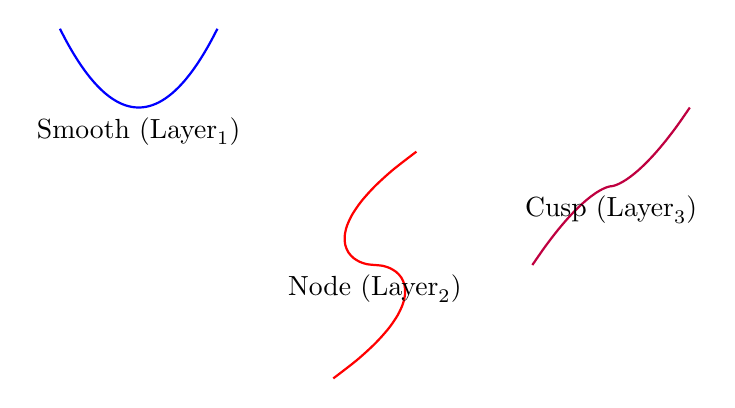
\begin{tikzpicture}
    % Smooth
    \draw[domain=-1:1, smooth, variable=\x, blue, thick] plot ({\x}, {\x*\x + 1});
    \node[below] at (0, 1) {Smooth ($\Layer{1}$)};
    
    % Node
    \begin{scope}[xshift=3cm]
        \draw[domain=-1.2:1.2, smooth, variable=\t, red, thick] plot ({\t^3-\t}, {\t^2-1});
        \node[below] at (0, -1) {Node ($\Layer{2}$)};
    \end{scope}
    
    % Cusp
    \begin{scope}[xshift=6cm]
        \draw[domain=-1:1, smooth, variable=\t, purple, thick] plot ({\t^2}, {\t^3});
        \node[below] at (0, 0) {Cusp ($\Layer{3}$)};
    \end{scope}
\end{tikzpicture}
\caption{曲線の特異点による階層化。構造塔の層が上がるほど、幾何学的な「悪さ（特異性）」が増していく。}
\end{figure}

% =========================================================================
% Section 4: 層理論とコホモロジー
% =========================================================================
\section{層 (Sheaf) とコホモロジー}

空間 $X$ 上の層 $\mathscr{F}$ を、その「広がり」や「コホモロジー的複雑さ」で分類する。

\subsection{層の台 (Support)}
層 $\mathscr{F}$ の台 $\mathrm{Supp}(\mathscr{F}) = \{x \in X \mid \mathscr{F}_x \neq 0\}$ の次元をランクとする。
\begin{itemize}
    \item $\MinLayer = 0$: Skyscraper sheaf（点層）。0次元の台を持つ。
    \item $\MinLayer = \dim X$: 構造層 $\mathcal{O}_X$ など。空間全体に広がる。
\end{itemize}

\subsection{コホモロジーの階層}
層 $\mathscr{F}$ が持つ非自明なコホモロジー群 $H^i(X, \mathscr{F})$ の最小次数 $i$ をランクとする考え方は、Serreの条件 $S_k$ やCohen-Macaulay性などのより高度な概念へと繋がる。

% =========================================================================
% Section 5: IUT理論への展望
% =========================================================================
\section{IUT理論への橋渡し：幾何的変形}

本課題の幾何的構造塔は、望月新一のIUT理論における以下の概念のモデルとなる。

\subsection{Hodge Theater と層の階層}
IUT理論では、異なる「宇宙（Hodge Theater）」の間で通信を行う。
構造塔の各層 $\Layer{n}$ は、ある一定の複雑さ（次元や高さ）以下の対象のみが存在する「部分宇宙」と見なせる。
例えば、$\Spec(\Z)$ の構造塔において、一般点 $(0)$ から閉点 $(p)$ への移行は、大域的な数体から局所体への移行（Localization）に対応し、これがIUTにおける \textbf{log-link} の原型となる。

\subsection{エタール被覆と遠アーベル幾何}
$\Spec(K)$ のエタール被覆の階層（例11）は、絶対ガロア群 $G_K$ の表現の階層に対応する。
Grothendieckの遠アーベル幾何予想は、この「被覆の塔（基本群）」の情報から、元の幾何的対象（曲線や数体）を復元できるかという問いであり、IUT理論はこの思想を極限まで推し進めたものである。

\begin{tcolorbox}[colback=green!5!white,colframe=green!75!black,title=学習のポイント]
「代数（数式）」と「幾何（図形）」は、双対的な関係にある。
\begin{itemize}
    \item 環の包含 $R \hookrightarrow S$ $\iff$ 空間の射 $\Spec(S) \to \Spec(R)$
    \item 素イデアルの高さ $\iff$ 空間の次元
    \item 剰余体による値の評価 $\iff$ 点における関数の値
\end{itemize}
この双対性を構造塔を通じて体感することが、現代数学（スキーム論）およびIUT理論への第一歩となる。
\end{tcolorbox}

\end{document}